\documentclass[12pt]{article}
%\usepackage{geometry}                % See geometry.pdf to learn the layout options. There are lots.
%\geometry{letterpaper}                   % ... or a4paper or a5paper or ... 
%\geometry{landscape}                % Activate for for rotated page geometry
\usepackage[parfill]{parskip}    % Activate to begin paragraphs with an empty line rather than an indent
\usepackage{daves,fancyhdr,natbib,graphicx,dcolumn,amsmath,lastpage,url}
\usepackage{amsmath,amssymb,epstopdf,longtable}
\usepackage{paralist}  % need to properly formulate standard answer blocks
\usepackage[final]{pdfpages}
\usepackage{multicol}
\usepackage{booktabs}
\DeclareGraphicsRule{.tif}{png}{.png}{`convert #1 `dirname #1`/`basename #1 .tif`.png}
\pagestyle{fancy}
\lhead{CE 3372 Water Systems Design; Exam 2}
\rhead{}%Name:\_\_\_\_\_\_\_\_\_\_\_\_\_\_\_\_\_\_\_\_\_\_\_\_\_\_\_\_\_\_\_\_\_\_}
\lfoot{SPRING 2025 REVISION 0}
\cfoot{}
\rfoot{Page \thepage\ of \pageref{LastPage}}
\renewcommand\headrulewidth{0pt}

%%%%%%%%%% Will's listing environment %%%%%%%
\usepackage[left=1.25in, right=1.25in,
            top=1in, bottom=1in]{geometry}                % See geometry.pdf to learn the layout options. There are lots.
\geometry{letterpaper}

\usepackage{ragged2e}

\usepackage{xcolor}
\newcommand{\codeRcolor}{0.93}
\newcommand{\codeGcolor}{0.93}
\newcommand{\codeBcolor}{0.93}
\definecolor{lightgrey}{rgb}{\codeRcolor,
                             \codeGcolor,
                             \codeBcolor}

\newcommand{\listingfont}{\fontsize{7pt}{8pt}\selectfont\ttfamily}
\usepackage{listings}
\lstset{basicstyle = \listingfont,
        breaklines = true,
        frame=tb,
        xleftmargin=12pt,
        framexleftmargin=6pt,
        framexrightmargin=6pt,
        xrightmargin=12pt,
        columns=fixed}
\lstset{lineskip=-1pt}
\lstset{backgroundcolor=\color{lightgrey}}


\usepackage[font={footnotesize},
            labelfont={sf,bf},
            textfont={sf},
            singlelinecheck=false,
            labelsep=none,
            justification=RaggedRight,
            aboveskip=0pt,
            belowskip=7pt plus 1pt minus 1pt,
            textformat=period]{caption}
\DeclareCaptionLabelSeparator{mystyle}{.\quad}
\captionsetup{labelsep=mystyle}
%%%%%%%%% End Will's listing environment ABOVE %%%%%%%%%
\newcommand\tab[1][1cm]{\hspace*{#1}}
\begin{document}
%%%%%%%%%%%%%%%%%%%%%%%%%%%%%%%%%%%
\begingroup
\begin{center}
{\textbf{{ CE 3372 Water Systems Design} \\ Exam 2 \\ Spring 2025} }
\end{center}
\endgroup

%Instructions: \\
%\begin{enumerate}
%\item Be sure to put your name on \textbf{each} sheet(including this one!).
%\item Choose the closest answer for questions with multiple choice answers; show work if you desire partial credit (e.g. arithmetic mistakes cost less if you include your work).
%\end{enumerate}
%\begin{tabular}{p{6in}}
%\hline \\
%\end{tabular}

\begin{enumerate}

%%%%%%%%%%%%%%%%%%%%%%%%%%%%%%%%%%%%%%%%%%%%
\item \label{prob:EPANET} (46 Points) Consider the pipe network portion shown in Figure \ref{fig:Pipes}.
\begin{quote}
The reservoir has a pool elevation of 1310 meters\\
\\
Node 1 elevation is 200.0 meters; Node 2 elevation is 150.0 meters\\
Node 3 elevation is 150.0 meters; Node 4 elevation is 100.0 meters\\
Node 5 elevation is 100.0 meters; Node 6 elevation is 50.0 meters\\
\\
P1 roughness is $e=0.045$ mm; P2  roughness is $e=0.045$ mm\\
P3 roughness is $e=0.045$ mm; P4  roughness is $e=0.090$ mm\\
P5 roughness is $e=0.045$ mm; P6  roughness is $e=0.045$ mm\\
P7 roughness is $e=0.045$ mm; P8  roughness is $e=0.045$ mm\\

\end{quote}
\begin{figure}[h!] %  figure placement: here, top, bottom, or page
\centering
   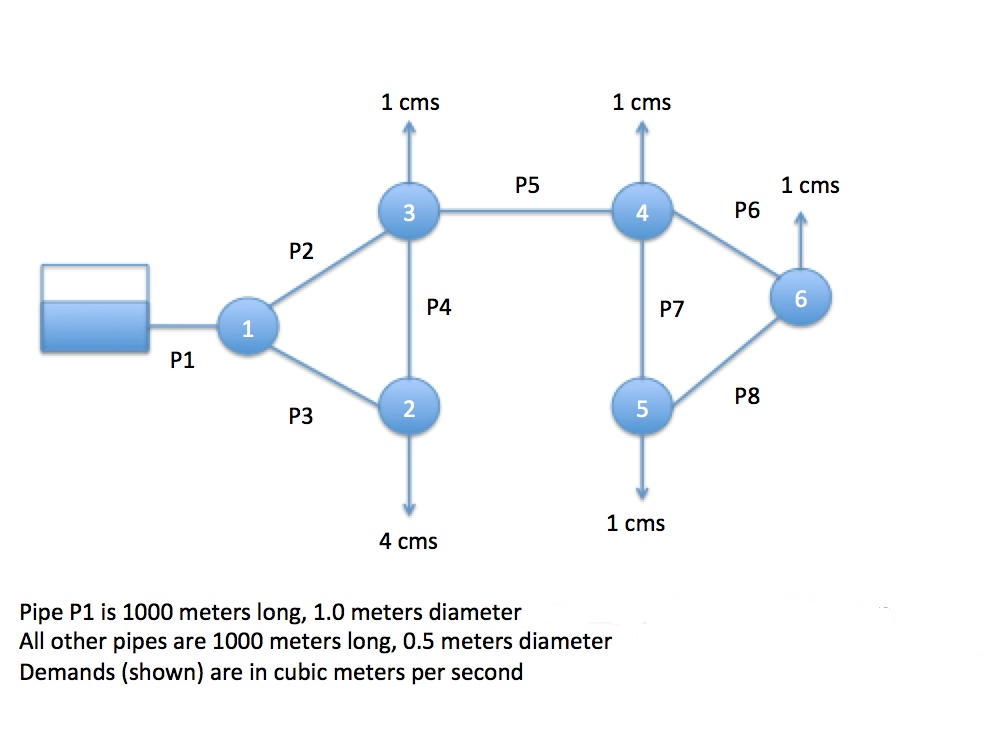
\includegraphics[width=6.5in]{2018Pipeline.jpg}
   \caption{Pipe Network}
   \label{fig:Pipes} 
\end{figure}
\clearpage

\begin{enumerate}[a)]
\item Use EPANET to determine the discharge, velocity, and head loss in each pipe and populate Table \ref{tab:pipes}

% Requires the booktabs if the memoir class is not being used
\begin{table}[htbp]
   %\centering
      \caption{Estimated $Q$,$V$, and $\Delta h$ in each pipe in Figure \ref{fig:Pipes} \\}
   %\topcaption{Table captions are better up top} % requires the topcapt package
   \begin{tabular}{| p{0.6in} | p{1.3in} | p{1.3in} | p{1.3in} |} % Column formatting, @{} suppresses leading/trailing space
   \hline
   \hline
Pipe ID & Discharge ($m^3/s$) & Velocity ($m/s$) & Head Loss ($m$)\\
\hline
\hline
1 &  ~ & ~ & ~ \\
~ &  ~ & ~ & ~ \\
~ &  ~ & ~ & ~ \\
\hline
2 &  ~ & ~ & ~ \\
~ &  ~ & ~ & ~ \\
~ &  ~ & ~ & ~ \\
\hline
3 &  ~ & ~ & ~ \\
~ &  ~ & ~ & ~ \\
~ &  ~ & ~ & ~ \\
\hline
4 &  ~ & ~ & ~ \\
~ &  ~ & ~ & ~ \\
~ &  ~ & ~ & ~ \\
\hline
5 &  ~ & ~ & ~ \\
~ &  ~ & ~ & ~ \\
~ &  ~ & ~ & ~ \\
\hline
6 &  ~ & ~ & ~ \\
~ &  ~ & ~ & ~ \\
~ &  ~ & ~ & ~ \\
\hline
7 &  ~ & ~ & ~ \\
~ &  ~ & ~ & ~ \\
~ &  ~ & ~ & ~ \\
\hline
8 &  ~ & ~ & ~ \\
~ &  ~ & ~ & ~ \\
~ &  ~ & ~ & ~ \\
\hline
\hline
   \end{tabular}
   \label{tab:pipes}
\end{table}

\clearpage
\item Use EPANET to determine the total head and pressure at each node and populate Table \ref{tab:booktabs} below.
% Requires the booktabs if the memoir class is not being used
\begin{table}[htbp]
   %\centering
      \caption{$TDH$, $z$,  and $P$ at  each node in Figure \ref{fig:Pipes} \\}
   %\topcaption{Table captions are better up top} % requires the topcapt package
   \begin{tabular}{| p{1in} | p{1.1in} | p{1in} | p{1.1in} | } % Column formatting, @{} suppresses leading/trailing space
   \hline
   \hline
Node ID & Total Head (m) & Elevation (m) & Pressure (kPa) \\
\hline
\hline
Reservoir & 1310 & N/A & 0  \\
~ & ~ & ~ & ~  \\
~ & ~ & ~ & ~  \\
\hline
1 & ~ & 200 & ~  \\
~ & ~ & ~ & ~  \\
~ & ~ & ~ & ~  \\
\hline
2 & ~ & 150 & ~  \\
~ & ~ & ~ & ~  \\
~ & ~ & ~ & ~  \\
\hline
3 & ~ & 150 & ~  \\
~ & ~ & ~ & ~  \\
~ & ~ & ~ & ~  \\
\hline
4 & ~ & 100 & ~  \\
~ & ~ & ~ & ~  \\
~ & ~ & ~ & ~  \\
\hline
5 & ~ & 100 & ~  \\
~ & ~ & ~ & ~  \\
~ & ~ & ~ & ~  \\
\hline
6 & ~ & 50 & ~  \\
~ & ~ & ~ & ~  \\
~ & ~ & ~ & ~  \\
\hline
\hline

   \end{tabular}

   \label{tab:booktabs}
\end{table}
\end{enumerate}


\begin{enumerate}[i)]
\item Attach a \textbf{screen capture} of your EPANET simulation here
\item Attach the EPANET \textbf{summary report} here
\end{enumerate}

\clearpage

%%%%%%%%%%%%%%%%%%%%%%%%%%%%%%%%%%%%%%%%%%%%%%
%%%%%%%% PROBLEM 1 %%%%%%%%%%%%%%%%%%%%%%%%%%%%%%%
%%%%%%%%%%%%%%%%%%%%%%%%%%%%%%%%%%%%%%%%%%%%%%
\item (1 points) The hydraulic radius in a conduit containing a flowing liquid is
\begin{enumerate} [(A)]
\item	the mean radius from the center of flow to the wetted side of the conduit
\item	the ratio of the cross-sectional area of the conduit and the wetted perimeter
\item	the ratio of the wetted perimeter and the cross-sectional area of the conduit
\item	the ratio of the cross-sectional area of flow and the wetted perimeter
\end{enumerate}
%%%%%%%%%%%%%%%%%%%%%%%%%%%%%%%%%%%%%%%%%%%%%%
%%%%%%%% PROBLEM 2 %%%%%%%%%%%%%%%%%%%%%%%%%%%%%%%
%%%%%%%%%%%%%%%%%%%%%%%%%%%%%%%%%%%%%%%%%%%%%%
\item (4 points) The rational runoff coefficient for a $14.81$~acre parcel property is $0.35$.  
The rainfall intensity is $4.56$ inches per hour.  
Determine the anticipated peak discharge from this property

% is anticipated to be about
%%standard answer set
%\begin{enumerate} [(A)]
%\item $22~ft^3/s$
%\item $24~ft^3/s$
%\item $38~ft^3/s$
%\item $70~ft^3/s$
%\item $22~ft^3/s$
%\item $24~ft^3/s$
%\item $38~ft^3/s$
%\item $70~ft^3/s$
%\end{enumerate}

\item (4 points) The rational runoff coefficient for a $300X200$-meter property with a slope of $3$\% is $0.35$.  The rainfall intensity is $116$ mm/hr.  Determine the anticipated peak discharge from this property

%The peak discharge from this property is anticipated to be about
%%standard answer set
%\begin{enumerate} [(A)]
%\item $2200~m^3/hr$
%\item $2400~m^3/hr$
%\item $3800~m^3/hr$
%\item $7000~m^3/hr$
%\end{enumerate}
%======== SOLUTION ===========
% B   Apply Rational Runoff Formula (in SI units)
% NCEES pp 159
%=============================
%
\item (5 points)  A storm sewer (reinforced concrete pipe) is 400-feet long and 30-inches in diameter.  The sewer flows from a junction box (invert elevation $101.00$ feet) to a lift station sump (invert elevation $100.00$ feet).  Assuming Manning's roughness coefficient is $0.013$ for all flow depths, determine the maximum sewer  flow capacity without surcharge 

%is about\footnote{For partial credit show work}
%% US Customary Versions
%\begin{enumerate} [(A)]
%\item  $17.8$ cfs
%\item  $19.2$ cfs
%\item  $20.6$ cfs
%\item  $22.1$ cfs
%\item  $28.9$ cfs
%\item  $31.2$ cfs
%\item  $33.4$ cfs
%\item  $35.9$ cfs
%\end{enumerate}
%%%%%%%%%%%%%%%%%%%%%%%%%%%%%%%
% n=0.013, So = 1/400, D = 30/12, Qf = 20.6 , Q= 22.1    % %
% n=0.013, So = 1/400, D = 36/12, Qf = 33.4 , Q = 35.9    % %
% n=0.015, So = 1/400, D = 30/12, Qf = 17.8 , Q= 19.1     %%
% n=0.015, So = 1/400, D = 36/12, Qf = 28.9 , Q = 31.2    %%
%%%%%%%%%%%%%%%%%%%%%%%%%%%%%%%


%%%%%%%%%%%%%%%%%%%%%%%%%%%%%%%%%%%%%%%%%%%%%%
%%%%%%%% PROBLEM 3 BEGIN %%%%%%%%%%%%%%%%%%%%%%%%%%%
%%%%%%%%%%%%%%%%%%%%%%%%%%%%%%%%%%%%%%%%%%%%%%
%====== SOLUTION ==========================
% C  use Manning's equation for full pipe flow
%  NCEES pp 160-161
%==========================================
%=======================================================================
%\clearpage
\item (5 points) The storm sewer in the question above is flowing at $\frac{3}{4}$ full.  What is the discharge in the sewer?
%standard answer set
%\begin{enumerate} [(A)]
%\item  $3.6$ cfs
%\item  $8.1$ cfs
%\item  $12.5$ cfs
%\item  $18.1$ cfs
%\item $22~ft^3/s$
%\item $24~ft^3/s$
%\item $38~ft^3/s$
%\item $70~ft^3/s$
%\end{enumerate}
%%%%%%%%%%%%%%%%%%%%%%%%%%%%%%%%%%%%%%%%%%%%%%
%%%%%%%% PROBLEM 4 DONE %%%%%%%%%%%%%%%%%%%%%%%%%%%
%%%%%%%%%%%%%%%%%%%%%%%%%%%%%%%%%%%%%%%%%%%%%%
\item  (5 points) A pipe with a diameter of $2.4$ meters is depicted in Figure \ref{fig:CircularSewerToo}.   The pipe is flowing partially full.

\begin{figure}[h!] %  figure placement: here, top, bottom, or page
\centering
   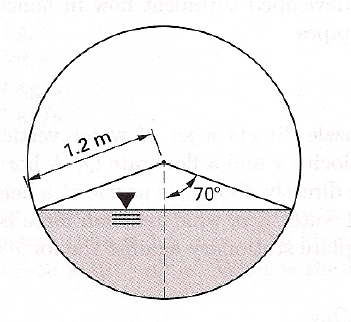
\includegraphics[width=1.9in]{CircularSewerToo.jpg}
   \caption{Circular channel flowing partially full.}
   \label{fig:CircularSewerToo} 
\end{figure}

Determine the hydraulic radius of flow in the circular section.
%%standard answer set
%\begin{enumerate} [(A)]
%\item $0.44$ m
%\item $0.88$ m
%\item $1.30$ m
%\item $1.80$ m
%\item $0.44$ m
%\item $0.88$ m
%\item $1.30$ m
%\item $1.80$ m
%\end{enumerate}
~\clearpage
\item  (5 points) A smooth concrete channel is depicted in Figure \ref{fig:TriangleChannel}.  The channel's dimensionless slope in the direction of flow is $0.005$.  The flow width at the surface is $2$-meters. 

%using the Hazen-Williams friction formula?

\begin{figure}[h!] %  figure placement: here, top, bottom, or page
\centering
   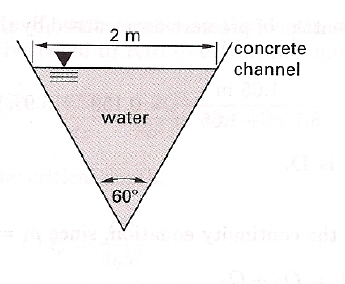
\includegraphics[width=2.2in]{TriangleChannel.jpg}
   \caption{Triangular channel.}
   \label{fig:TriangleChannel} 
\end{figure}

Determine the flow rate in the channel.

%%standard answer set
%\begin{enumerate} [(A)]
%\item $0.80~ m^3/sec$
%\item $1.30~ m^3/sec$
%\item $1.45~ m^3/sec$
%\item $2.20~ m^3/sec$
%\item $22~ft^3/s$
%\item $24~ft^3/s$
%\item $38~ft^3/s$
%\item $70~ft^3/s$
%\end{enumerate}

%%%%%%%%%%%%%%%%%%%%%%%%%%%%%%%%%%%%%%%%%%%%%%
%%%%%%%% PROBLEM 6 BEGIN %%%%%%%%%%%%%%%%%%%%%%%%%%%
%%%%%%%%%%%%%%%%%%%%%%%%%%%%%%%%%%%%%%%%%%%%%%
%\clearpage
\item (10 points) A 24-inch diameter sewer pipe, with Manning's n of $0.015$ is laid on slope $S_0 =0.01$ as shown in Figure \ref{fig:PipeOnSlope}.    

\begin{figure}[h!] %  figure placement: here, top, bottom, or page
\centering
   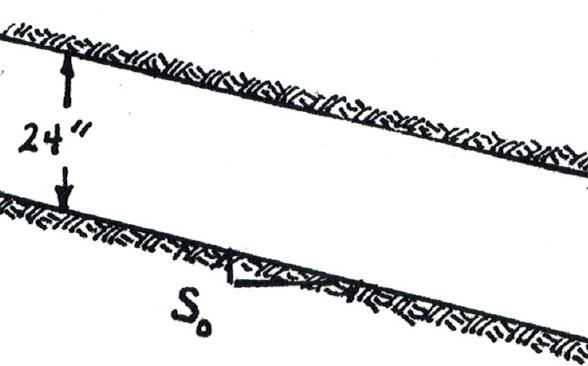
\includegraphics[width=2in]{PipeOnSlope.jpg}
   \caption{Sewer pipe sketch}
   \label{fig:PipeOnSlope} 
\end{figure}

Use Manning's equation and the depth-area, and the depth-perimeter equations to complete Table \ref{tab:SewerPipes}.
% Requires the booktabs if the memoir class is not being used
\begin{table}[htbp]
   \centering
   \caption{Depth-Area, Depth-Perimeter, Depth-Hyd. Radius, and Discharge for Circular Sewer}
   \begin{tabular}{p{1in}p{1in}p{1in}p{1in}p{1in}}
   ~ & ~ & ~  & ~ & ~ \\
$y$ ($ft$)~~& $A$ ($ft^2$) & $P_w$ ($ft$) & $R_h$ ($ft$) & $Q$ ($ft^3/sec$) \\
\hline
\hline
~ & ~ & ~  & ~ & ~ \\
1.00 & ~ & ~  & ~ & ~ \\
~& ~ & ~  & ~ & ~ \\
\hline
~ & ~ & ~  & ~ & ~ \\
2.00 & ~ & ~  & ~ & ~ \\
~ & ~ & ~  & ~ & ~ \\
\hline
   \end{tabular}
   \label{tab:SewerPipes}
\end{table}

\clearpage

%%%%%%%%%%%%%%%%%%%%%%%%%%%%%%%%%%%%%%%%%%%%
\item \label{prob:DrainDesign1} (15 points)Consider the drainage area depicted in Figure \ref{fig:DrainageCase1}.  The 6.0 acre drainage area has a runoff coefficient of 0.65, and an inlet time (time of concentration to the inlet depicted in the figure) of 17 minutes.  The pipes are concrete (Manning's $n$ = 0.013).  The initial invert elevations for the junction boxes (MH-1, MH-2, MH-3) are 323.2, 321.1, and 319.0 feet, respectively.

\begin{figure}[ht!] %  figure placement: here, top, bottom, or page
\centering
   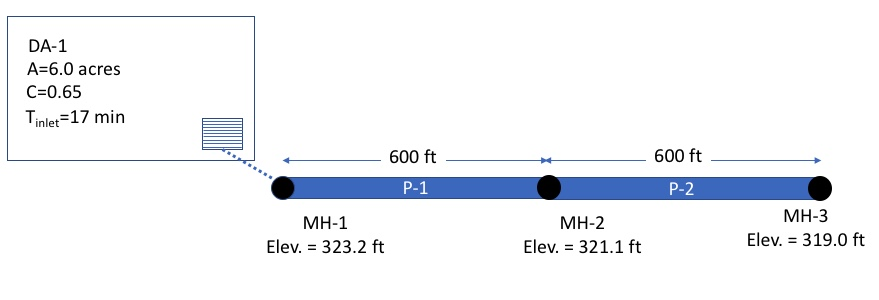
\includegraphics[width=6in]{DrainageCase1.jpg}
   \caption{Drainage System Layout}
   \label{fig:DrainageCase1} 
\end{figure}
Equation \ref{eqn:intensity1} is the 10-year ARI intensity equation for the area, where $I$ is intensity in inches-per-hour, and $T_c$ is the characteristic time, in minutes.

\begin{equation}
I = \frac{56.6}{(T_c + 8.6)^{0.823}}
\label{eqn:intensity1}
\end{equation}

%Questions related to the drainage design begin on the next page.
%~\\
%\begin{tabular}{p{6in}}
%~\\
%\hline
%\end{tabular}
%\clearpage
\begin{enumerate}[a)]
\item What is the dimensionless slope of the pipe run P1 (connecting MH-1 and MH-2)? ~\\~\\
\item What is the dimensionless slope of the pipe run P2 (connecting MH-2 and MH-3)?  ~\\~\\
\item What is the $CA$ value for drainage area DA-1?  ~\\~\\
\item What is the $\sum{CA}$ value (sum of the upstream products of runoff coefficients and contributing areas) at junction MH-1?  ~\\~\\
\item What is the $\sum{CA}$ value (sum of the upstream products of runoff coefficients and contributing areas) at junction MH-2?  ~\\~\\
\item What is the time of concentration to be used to compute the discharge leaving MH-1?  ~\\~\\
\item What is the rainfall intensity for this time of concentration?  ~\\~\\
\item What is the value of peak discharge leaving MH-1?  ~\\~\\
\item What is the pipe diameter for pipe P-1 required the carry the design flow at full pipe depth?  ~\\~\\
\item What is the flow velocity in pipe P-1?  ~\\~\\
\item What is the pipe travel time for pipe P-1?  ~\\~\\
\item What is the value of peak discharge leaving MH-2? (Explain your reasoning)  ~\\~\\
\item What is the pipe diameter for pipe P-2 required the carry the design flow at full pipe depth?  ~\\~\\
\item What is the flow velocity in pipe P-2?  ~\\~\\
\item What is the pipe travel time for  pipe P-2?  ~\\~\\
\end{enumerate}
\clearpage

%\item \label{prob:DrainDesign2} Consider the drainage area depicted in Figure \ref{fig:DrainageCase2}.  Drainage area DA-1 is a 6.0 acre drainage area has a runoff coefficient of 0.65, and an inlet time (time of concentration to the inlet depicted in the figure) of 17 minutes.  
%Drainage area DA-2 is a 5.1 acre drainage area has a runoff coefficient of 0.55, and an inlet time (time of concentration to the inlet depicted in the figure) of 14 minutes.
%The pipes, P-1 and P-2 are concrete (Manning's $n$ = 0.013).  
%The initial invert elevations for the junction boxes (MH-1, MH-2, MH-3) are 323.2, 321.1, and 319.0 feet, respectively.
%
%\begin{figure}[ht!] %  figure placement: here, top, bottom, or page
%\centering
%   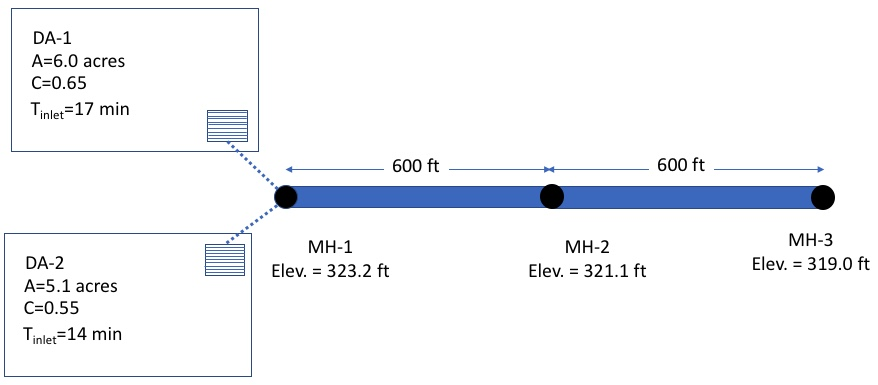
\includegraphics[width=6in]{DrainageCase2.jpg}
%   \caption{Drainage System Layout}
%   \label{fig:DrainageCase2} 
%\end{figure}
%Equation \ref{eqn:intensity2} is the 10-year ARI intensity equation for the area, where $I$ is intensity in inches-per-hour, and $T_c$ is the characteristic time, in minutes.
%
%\begin{equation}
%I = \frac{56.6}{(T_c + 8.6)^{0.823}}
%\label{eqn:intensity2}
%\end{equation}
%%~\\
%%\begin{tabular}{p{6in}}
%%~\\
%%\hline
%%\end{tabular}
%\begin{enumerate}[a)]
%\item What is the dimensionless slope of the pipe run P1 (connecting MH-1 and MH-2)? ~\\
%\item What is the dimensionless slope of the pipe run P2 (connecting MH-2 and MH-3)? ~\\
%\item What is the $CA$ value for drainage area DA-1? ~\\
%\item What is the $CA$ value for drainage area DA-2? ~\\
%\item What is the $\sum{CA}$ value (sum of the upstream products of runoff coefficients and contributing areas) at junction MH-1? ~\\
%\item What is the $\sum{CA}$ value (sum of the upstream products of runoff coefficients and contributing areas) at junction MH-2? ~\\~\\
%\item What is the time of concentration to be used to compute the discharge leaving MH-1? ~\\~\\
%\item What is the rainfall intensity for this time of concentration? ~\\~\\
%\item What is the value of peak discharge leaving MH-1? ~\\~\\
%\item What is the pipe diameter for pipe P-1 required the carry the design flow at full pipe depth? ~\\~\\
%\item What is the flow velocity in pipe P-1? ~\\~\\
%\item What is the pipe travel time for pipe P-1?~\\~\\
%\item What is the value of peak discharge leaving MH-2? (Explain your reasoning) ~\\~\\
%\item What is the pipe diameter for pipe P-2 required the carry the design flow at full pipe depth? ~\\~\\
%\item What is the flow velocity in pipe P-2? ~\\~\\
%\item What is the pipe travel time for  pipe P-2?
%\end{enumerate}
%\clearpage
%
%\item \label{prob:DrainDesign3} Consider the drainage area depicted in Figure \ref{fig:DrainageCase3}.  
%Drainage area DA-1 is a 6.0 acre drainage area has a runoff coefficient of 0.65, and an inlet time (time of concentration to the inlet depicted in the figure) of 17 minutes.  
%Drainage area DA-2 is a 5.1 acre drainage area has a runoff coefficient of 0.55, and an inlet time (time of concentration to the inlet depicted in the figure) of 14 minutes.
%Drainage area DA-3 is a 3.5 acre drainage area has a runoff coefficient of 0.70, and an inlet time (time of concentration to the inlet depicted in the figure) of 12 minutes.
%The pipes, P-1 and P-2 are concrete (Manning's $n$ = 0.013).  
%The initial invert elevations for the junction boxes (MH-1, MH-2, MH-3) are 323.2, 321.1, and 319.0 feet, respectively.
%
%\begin{figure}[ht!] %  figure placement: here, top, bottom, or page
%\centering
%   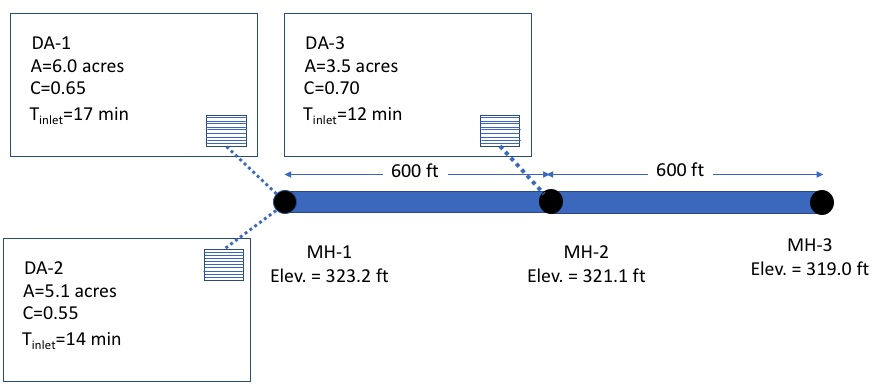
\includegraphics[width=6in]{DrainageCase3.jpg}
%   \caption{Drainage System Layout}
%   \label{fig:DrainageCase3} 
%\end{figure}
%Equation \ref{eqn:intensity3} is the 10-year ARI intensity equation for the area, where $I$ is intensity in inches-per-hour, and $T_c$ is the characteristic time, in minutes.
%
%\begin{equation}
%I = \frac{56.6}{(T_c + 8.6)^{0.823}}
%\label{eqn:intensity3}
%\end{equation}
%%~\\
%%\begin{tabular}{p{6in}}
%%~\\
%%\hline
%%\end{tabular}
%\begin{enumerate}[a)]
%\item What is the dimensionless slope of the pipe run P1 (connecting MH-1 and MH-2)? ~\\~\\
%\item What is the dimensionless slope of the pipe run P2 (connecting MH-2 and MH-3)? ~\\~\\ ~\newpage
%\item What is the $CA$ value for drainage area DA-1? ~\\~\\
%\item What is the $CA$ value for drainage area DA-2? ~\\~\\
%\item What is the $CA$ value for drainage area DA-3? ~\\~\\
%\item What is the $\sum{CA}$ value (sum of the upstream products of runoff coefficients and contributing areas) at junction MH-1? ~\\~\\
%\item What is the $\sum{CA}$ value (sum of the upstream products of runoff coefficients and contributing areas) at junction MH-2? ~\\~\\
%\item What is the time of concentration to be used to compute the discharge leaving MH-1? ~\\~\\
%\item What is the rainfall intensity for this time of concentration? ~\\~\\
%\item What is the value of peak discharge leaving MH-1? ~\\~\\
%\item What is the pipe diameter for pipe P-1 required the carry the design flow at full pipe depth?~\\~\\
%\item What is the flow velocity in pipe P-1?~\\~\\
%\item What is the pipe travel time for pipe P-1?~\\~\\ 
%\item What is the time of concentration to be used to compute the discharge leaving MH-2? ~\\~\\
%\item What is the rainfall intensity for this time of concentration? ~\\~\\
%\item What is the value of peak discharge leaving MH-2? ~\\~\\
%\item What is the pipe diameter for pipe P-2 required the carry the design flow at full pipe depth?~\\~\\
%\item What is the flow velocity in pipe P-2?~\\~\\
%\item What is the pipe travel time for pipe P-2?
%\end{enumerate}
%\clearpage
%
%\item \label{prob:FlowDepth}
%Using the pipe sizes you determined in Problem \ref{prob:DrainDesign3}, resize the pipes so the pipes convey the design flows at 1/2 full. Round your results up to the nearest 0.1 foot value.
%\begin{figure}[h!] %  figure placement: here, top, bottom, or page
%\centering
%   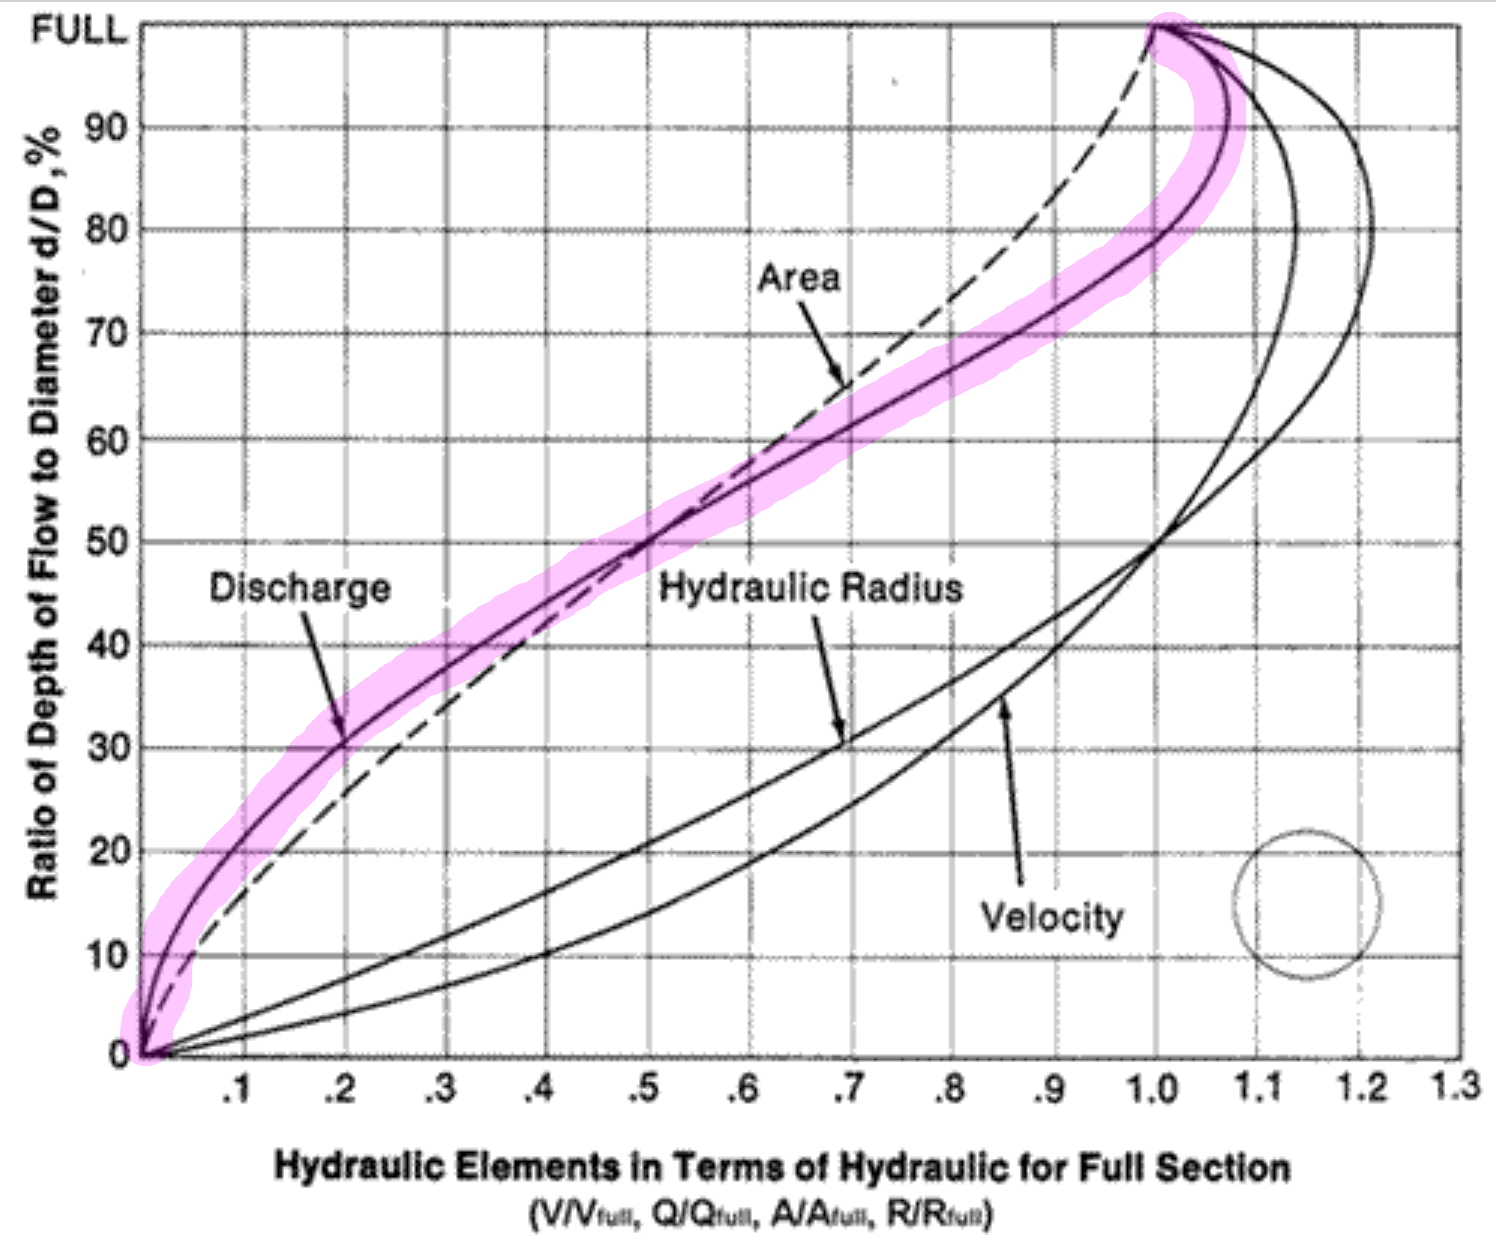
\includegraphics[height=5in]{hydraulic-elements-simple.jpg}
%   \caption{Hydraulic elements chart}
%   \label{fig:hydraulic-elements-simple} 
%\end{figure}
%~\\~\\~\\~\\~\\~\\~\\~\\~\\~\\
%\begin{enumerate}[a)]
%\item Diameter P-1 =
%\item Diameter P-2 =
%\end{enumerate}
%\clearpage
%
%\item \label{prob:DrainDesignReset}
%Using the pipe sizes you determined in Problem \ref{prob:FlowDepth}, determine the required invert elevations of junction boxes MH-1 and MH-2 that maintain the pipe slopes of pipes P-1 and P-2, maintain the junction box elevation of MH-3, and match soffit elevations (top of pipe) at each junction.  Make an elevation view sketch of the conduit system.
%~\\~\\~\\~\\~\\~\\~\\~\\~\\~\\~\\~\\~\\~\\~\\~\\~\\~\\~\\~\\
%
%%%%%%%%%%%%%%%%%%%%%%%%%%%%%%%%%%%%%%%%%%%%%%%%%%%%%%
%%%%%%PROBLEM 6 SWMM INTERPRETATION %%%%%%%%%%%%%%%%%%%%%%%%%%%
%%%%%%%%%%%%%%%%%%%%%%%%%%%%%%%%%%%%%%%%%%%%%%%%%%%%%%

%\item (32 points) Listing \ref{lst:SWMM Input} is a SWMM input file listing, and Listing \ref{lst:SWMM Summary} is a SWMM summary file for a particular sewer system.   
%Using these files answer the following questions:~\\
%\begin{enumerate}[a)]
%\item How many sub-catchments are modeled?~\\
%\item How many outfalls are modeled?~\\
%\item How many conduits are modeled?~\\
%\item What is the peak intensity of the design storm applied in the SWMM model ?~\\
%\item How long is the storm applied to the drainage system?~\\
%\item How long is the drainage system simulation run? \\
%\item What is the maximum discharge from the system in cubic feet per second?~\\
%\item What is the diameter in inches of the most downstream conduit?~\\
%\item How many junctions are modeled?~\\
%\item Are any of the conduits offset relative to a connecting junction?
%~\\
%
%
%\item Which drawing in Figure \ref{fig:boundary-condition} is representative of the downstream (outfall) boundary condition in the SWMM model?
%\begin{figure}[ht!] %  figure placement: here, top, bottom, or page
%\centering
%   \includegraphics[width=6in]{boundary-condition.pdf}
%   \caption{Conceptual downstream boundary conditions}
%   \label{fig:boundary-condition} 
%\end{figure}
%
%\item Which conduit had the largest peak flow?~\\
%\item Which conduit had the smallest peak flow?~\\
%\item What was the depth of water in the conduit with the smallest flow (in feet)?~\\
%\item What was the depth of water in the conduit with the largest flow (in feet)?~\\
%\item What was the total runoff, in watershed inches, for the model?~\\
%\item What hydrologic method was used in the model?~\\
%\item What flow routing method was used in the model?~\\
%\item What was the run date of the model?~\\
%\item What version number and build number of SWMM was used in the model?~\\
%\end{enumerate}
%\clearpage
%

%standard answer set


%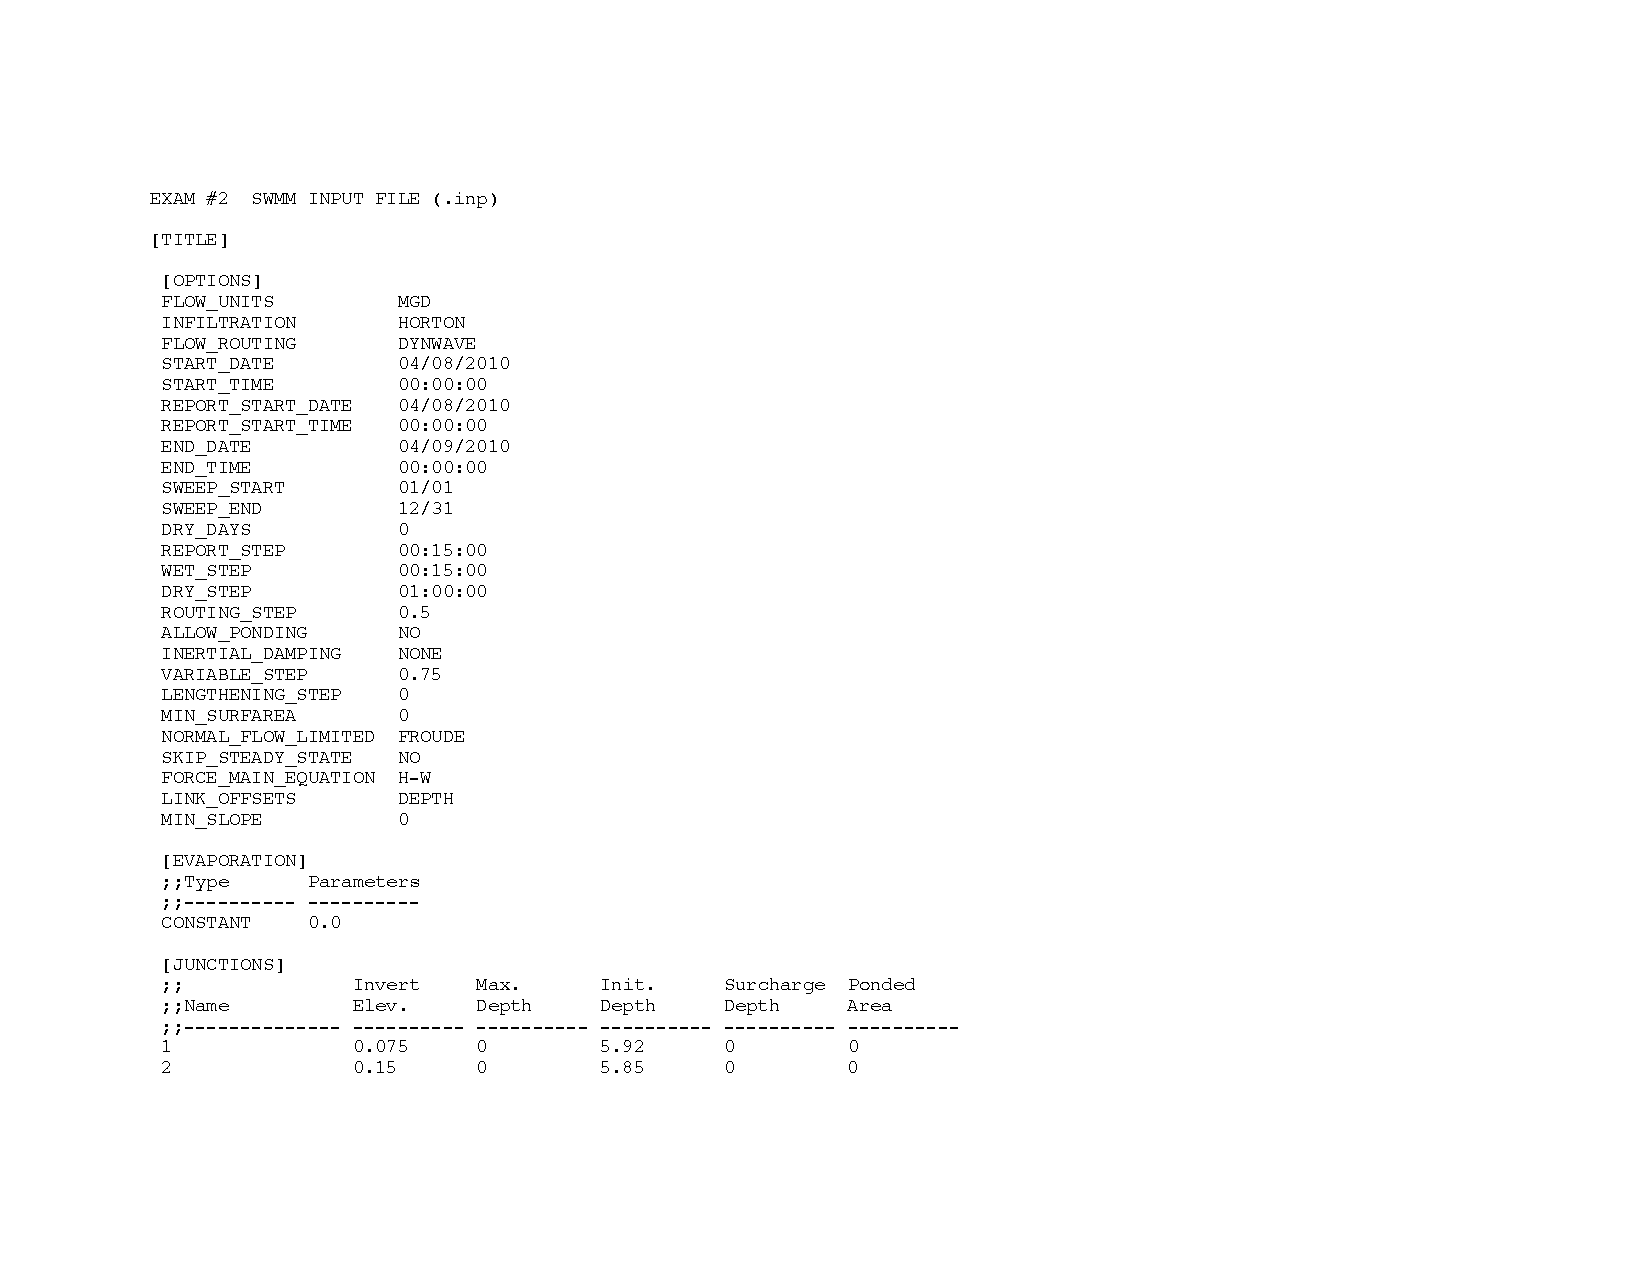
\includepdf[pages=-]{SWMM.pdf}

\end{enumerate}

%\begin{lstlisting}[caption=SWMM Input File Listing, label=lst:SWMM Input]
%[TITLE]
%;;Project Title/Notes
%[OPTIONS]
%;;Option             Value
%FLOW_UNITS           CFS
%INFILTRATION         HORTON
%FLOW_ROUTING         KINWAVE
%LINK_OFFSETS         DEPTH
%MIN_SLOPE            0
%ALLOW_PONDING        NO
%SKIP_STEADY_STATE    NO
%START_DATE           04/26/2017
%START_TIME           00:00:00
%REPORT_START_DATE    04/26/2017
%REPORT_START_TIME    00:00:00
%END_DATE             04/26/2017
%END_TIME             06:00:00
%SWEEP_START          01/01
%SWEEP_END            12/31
%DRY_DAYS             0
%REPORT_STEP          00:01:00
%WET_STEP             00:01:00
%DRY_STEP             01:00:00
%ROUTING_STEP         0:00:30 
%INERTIAL_DAMPING     PARTIAL
%NORMAL_FLOW_LIMITED  BOTH
%FORCE_MAIN_EQUATION  H-W
%VARIABLE_STEP        0.75
%LENGTHENING_STEP     0
%MIN_SURFAREA         12.557
%MAX_TRIALS           8
%HEAD_TOLERANCE       0.005
%SYS_FLOW_TOL         5
%LAT_FLOW_TOL         5
%[EVAPORATION]
%;;Evap Data      Parameters
%;;-------------- ----------------
%CONSTANT         0.0
%DRY_ONLY         NO
%[RAINGAGES]
%;;Gage           Format    Interval SCF      Source    
%;;-------------- --------- ------ ------ ----------
%1                INTENSITY 1:00     1.0      TIMESERIES DESIGN-STORM    
%[SUBCATCHMENTS]
%;;Subcatchment   Rain Gage        Outlet           Area     %Imperv  Width    %Slope        
%;;-------------- ---------------- ---------------- -------- -------- -------- -------- 
%1                1                4                6        65       2500     0.5                              
%2                1                4                5.1      55       2000     0.5                              
%3                1                5                3.5      70       2000     0.5                              
%[SUBAREAS]
%;;Subcatchment   N-Imperv   N-Perv     S-Imperv   S-Perv     PctZero    RouteTo    
%;;-------------- ---------- ---------- ---------- ---------- ---------- ---------- 
%1                0.01       0.1        0.05       0.05       25         OUTLET    
%2                0.01       0.1        0.05       0.05       25         OUTLET    
%3                0.01       0.1        0.05       0.05       25         OUTLET    
%[INFILTRATION]
%;;Subcatchment   MaxRate    MinRate    Decay      DryTime    MaxInfil  
%;;-------------- ---------- ---------- ---------- ---------- ----------
%1                10         6          4          7          0         
%2                12         6          4          7          0         
%3                12         6          4          7          0         
%[JUNCTIONS]
%;;Junction       Invert     MaxDepth   InitDepth  SurDepth   Aponded   
%;;-------------- ---------- ---------- ---------- ---------- ----------
%4                6.34       10         0          0          0         
%5                3.92       10         0          0          0         
%6                2          10         0          0          0         
%[OUTFALLS]
%;;Outfall        Invert     Type       Stage Data       Gated   
%;;-------------- ---------- ---------- ---------------- --------
%7                0          FREE                        NO
%[CONDUITS]
%;;Conduit     From    To      Length  Roughness  InOffset OutOffset InitFlow MaxFlow  
%              Node    Node                 
%;;-------- ---------- ---------- ------- ------- ------- -------    -------  -------  
%2            5            6       600    0.013      0       0       0          0  
%1            4            5       600    0.013      0       .5      0          0         
%3            6            7       600    0.013      0       0       0          0         
%[XSECTIONS]
%;;Link           Shape        Geom1            Geom2      Geom3      Geom4      Barrels   
%;;-------------- ------------ ---------------- ---------- ---------- ---------- ----------
%2                CIRCULAR     3.5              0          0          0          1   
%1                CIRCULAR     3                0          0          0          1                    
%3                CIRCULAR     3.5              0          0          0          1                    
%[TIMESERIES]
%;;Time Series    Date       Time       Value     
%;;-------------- ---------- ---------- ----------
%DESIGN-STORM                0          4.4       
%DESIGN-STORM                1          4.4       
%DESIGN-STORM                2          4.4       
%DESIGN-STORM                3          4.4       
%DESIGN-STORM                4          0         
%DESIGN-STORM                5          0         
%DESIGN-STORM                6          0         
%DESIGN-STORM                7          0         
%[REPORT]
%;;Reporting Options
%INPUT      NO
%CONTROLS   NO
%SUBCATCHMENTS ALL
%NODES ALL
%LINKS ALL
%[TAGS]
%[MAP]
%DIMENSIONS 0.000 0.000 10000.000 10000.000
%Units      None
%[COORDINATES]
%;;Node           X-Coord            Y-Coord           
%;;-------------- ------------------ ------------------
%4                -371.901           8402.204          
%5                1584.022           8388.430          
%6                3415.978           8415.978          
%7                5234.160           8429.752          
%[VERTICES]
%;;Link           X-Coord            Y-Coord           
%;;-------------- ------------------ ------------------
%[Polygons]
%;;Subcatchment   X-Coord            Y-Coord           
%;;-------------- ------------------ ------------------
%1                -2162.534          9242.424          
%1                -633.609           9228.650          
%1                -647.383           8484.848          
%1                -2162.534          8512.397          
%1                -2148.760          9256.198          
%2                -2148.760          8319.559          
%2                -647.383           8333.333          
%2                -688.705           7617.080          
%2                -2176.309          7603.306          
%2                -2176.309          8388.430          
%3                -96.419            9228.650          
%3                1528.926           9228.650          
%3                1460.055           8457.300          
%3                -165.289           8484.848          
%3                -110.193           9201.102          
%[SYMBOLS]
%;;Gage           X-Coord            Y-Coord           
%;;-------------- ------------------ ------------------
%1                -2231.405          9641.873  
%\end{lstlisting}  
%
%\begin{lstlisting}[caption=SWMM Output Summary File Listing, label=lst:SWMM Summary]
% EPA STORM WATER MANAGEMENT MODEL - VERSION 5.1 (Build 5.1.007)
%  --------------------------------------------------------------
%  *********************************************************
%  NOTE: The summary statistics displayed in this report are
%  based on results found at every computational time step,  
%  not just on results from each reporting time step.
%  *********************************************************
%  ****************
%  Analysis Options
%  ****************
%  Flow Units ............... CFS
%  Process Models:
%    Rainfall/Runoff ........ YES
%    RDII ................... NO
%    Snowmelt ............... NO
%    Groundwater ............ NO
%    Flow Routing ........... YES
%    Ponding Allowed ........ NO
%    Water Quality .......... NO
%  Infiltration Method ...... HORTON
%  Flow Routing Method ...... KINWAVE
%  Starting Date ............ APR-26-2017 00:00:00
%  Ending Date .............. APR-26-2017 06:00:00
%  Antecedent Dry Days ...... 0.0
%  Report Time Step ......... 00:01:00
%  Wet Time Step ............ 00:01:00
%  Dry Time Step ............ 01:00:00
%  Routing Time Step ........ 30.00 sec
%  Variable Time Step ....... YES
%  Maximum Trials ........... 8
%  Head Tolerance ........... 0.005000 ft
%  **************************        Volume         Depth
%  Runoff Quantity Continuity     acre-feet        inches
%  **************************     ---------       -------
%  Total Precipitation ......        21.413        17.600
%  Evaporation Loss .........         0.000         0.000
%  Infiltration Loss ........         7.986         6.564
%  Surface Runoff ...........        13.402        11.015
%  Final Surface Storage ....         0.029         0.024
%  Continuity Error (%) .....        -0.018
%  **************************        Volume        Volume
%  Flow Routing Continuity        acre-feet      10^6 gal
%  **************************     ---------     ---------
%  Dry Weather Inflow .......         0.000         0.000
%  Wet Weather Inflow .......        13.402         4.367
%  Groundwater Inflow .......         0.000         0.000
%  RDII Inflow ..............         0.000         0.000
%  External Inflow ..........         0.000         0.000
%  External Outflow .........        13.396         4.365
%  Internal Outflow .........         0.000         0.000
%  Evaporation Loss .........         0.000         0.000
%  Exfiltration Loss ........         0.000         0.000
%  Initial Stored Volume ....         0.000         0.000
%  Final Stored Volume ......         0.001         0.000
%  Continuity Error (%) .....         0.043
%  ***************************
%  Time-Step Critical Elements
%  ***************************
%  None
%  ********************************
%  Highest Flow Instability Indexes
%  ********************************
%  All links are stable.
%  *************************
%  Routing Time Step Summary
%  *************************
%  Minimum Time Step           :    30.00 sec
%  Average Time Step           :    29.96 sec
%  Maximum Time Step           :    30.00 sec
%  Percent in Steady State     :     0.00
%  Average Iterations per Step :     2.08
%  Percent Not Converging      :     0.14
%  ***************************
%  Subcatchment Runoff Summary
%  ***************************
%  --------------------------------------------------------------------------------------------------------
%                            Total      Total      Total      Total      Total       Total     Peak  Runoff
%                           Precip      Runon       Evap      Infil     Runoff      Runoff   Runoff   Coeff
%  Subcatchment                 in         in         in         in         in    10^6 gal      CFS
%  --------------------------------------------------------------------------------------------------------
%  1                         17.60       0.00       0.00       6.16      11.42        1.86    17.30   0.649
%  2                         17.60       0.00       0.00       7.92       9.66        1.34    12.45   0.549
%  3                         17.60       0.00       0.00       5.28      12.30        1.17    10.87   0.699
%  ******************
%  Node Depth Summary
%  ******************
%  ---------------------------------------------------------------------
%                                 Average  Maximum  Maximum  Time of Max
%                                   Depth    Depth      HGL   Occurrence
%  Node                 Type         Feet     Feet     Feet  days hr:min
%  ---------------------------------------------------------------------
%  4                    JUNCTION     1.37     2.01     8.35     0  00:44
%  5                    JUNCTION     1.49     2.19     6.11     0  00:09
%  6                    JUNCTION     1.47     2.16     4.16     0  00:10
%  7                    OUTFALL      1.35     1.99     1.99     0  00:11
%  *******************
%  Node Inflow Summary
%  *******************
%  -------------------------------------------------------------------------------------------------
%                                  Maximum  Maximum                  Lateral       Total        Flow
%                                  Lateral    Total  Time of Max      Inflow      Inflow     Balance
%                                   Inflow   Inflow   Occurrence      Volume      Volume       Error
%  Node                 Type           CFS      CFS  days hr:min    10^6 gal    10^6 gal     Percent
%  -------------------------------------------------------------------------------------------------
%  4                    JUNCTION     29.75    29.75     0  00:45         3.2         3.2       0.026
%  5                    JUNCTION     10.87    40.62     0  00:46        1.17        4.37       0.001
%  6                    JUNCTION      0.00    40.62     0  00:23           0        4.37       0.027
%  7                    OUTFALL       0.00    40.81     0  00:11           0        4.36       0.000
%  **********************
%  Node Surcharge Summary
%  **********************
%  No nodes were surcharged.
%  *********************
%  Node Flooding Summary
%  *********************
%  No nodes were flooded.
%  ***********************
%  Outfall Loading Summary
%  ***********************
%  -----------------------------------------------------------
%                         Flow       Avg       Max       Total
%                         Freq      Flow      Flow      Volume
%  Outfall Node           Pcnt       CFS       CFS    10^6 gal
%  -----------------------------------------------------------
%  7                     99.86     27.02     40.81       4.365
%  -----------------------------------------------------------
%  System                99.86     27.02     40.81       4.365
%  ********************
%  Link Flow Summary
%  ********************
%  -----------------------------------------------------------------------------
%                                 Maximum  Time of Max   Maximum    Max/    Max/
%                                  |Flow|   Occurrence   |Veloc|    Full    Full
%  Link                 Type          CFS  days hr:min    ft/sec    Flow   Depth
%  -----------------------------------------------------------------------------
%  2                    CONDUIT     40.62     0  00:23      7.03    0.71    0.62
%  1                    CONDUIT     29.75     0  00:45      6.37    0.79    0.63
%  3                    CONDUIT     40.81     0  00:11      6.89    0.70    0.59
%  
%  ***************************
%  Flow Classification Summary
%  ***************************
%  -------------------------------------------------------------------------------------
%                      Adjusted    ---------- Fraction of Time in Flow Class ---------- 
%                       /Actual         Up    Down  Sub   Sup   Up    Down  Norm  Inlet 
%  Conduit               Length    Dry  Dry   Dry   Crit  Crit  Crit  Crit  Ltd   Ctrl  
%  -------------------------------------------------------------------------------------
%  2                       1.00   0.00  0.00  0.00  0.98  0.02  0.00  0.00  0.33  0.00
%  1                       1.00   0.00  0.00  0.00  0.00  0.00  0.00  1.00  0.00  0.00
%  3                       1.00   0.00  0.00  0.00  0.80  0.20  0.00  0.00  0.02  0.00
%  *************************
%  Conduit Surcharge Summary
%  *************************
%  No conduits were surcharged.
%  Analysis begun on:  Wed Apr 26 19:29:56 2017
%  Analysis ended on:  Wed Apr 26 19:29:56 2017
%  Total elapsed time: < 1 sec
%\end{lstlisting}  
%\clearpage
%List your team members names below.
%For each team member assess their performance.  Consider their actual participation, their timeliness at completing assignment tasks, their reliability on completing assignment tasks.   Also state (1) whether you would be willing to work with them again on team assignments, and (2) whether you would recommend them to a friend who is trying to assemble a team for a future class.
%\begin {enumerate} [1)]
%\item \_\_\_\_\_\_\_\_\_\_\_\_\_\_\_\_\_\_\_\_\_\_\_\_\_\_\_\_\_\_\_\_\_\_\_\_\_\_\_\_\_\_\_\_\_\_\_\_\_\_\_\_\_\_\_\_\_\_\_\_\_\_\_\_\_\_ 
%~\\~\\~\\~\\~\\~\\
%\item \_\_\_\_\_\_\_\_\_\_\_\_\_\_\_\_\_\_\_\_\_\_\_\_\_\_\_\_\_\_\_\_\_\_\_\_\_\_\_\_\_\_\_\_\_\_\_\_\_\_\_\_\_\_\_\_\_\_\_\_\_\_\_\_\_\_ ~\\
%~\\~\\~\\~\\~\\~\\
%\item \_\_\_\_\_\_\_\_\_\_\_\_\_\_\_\_\_\_\_\_\_\_\_\_\_\_\_\_\_\_\_\_\_\_\_\_\_\_\_\_\_\_\_\_\_\_\_\_\_\_\_\_\_\_\_\_\_\_\_\_\_\_\_\_\_\_ ~\\
%~\\~\\~\\~\\~\\~\\
%\item \_\_\_\_\_\_\_\_\_\_\_\_\_\_\_\_\_\_\_\_\_\_\_\_\_\_\_\_\_\_\_\_\_\_\_\_\_\_\_\_\_\_\_\_\_\_\_\_\_\_\_\_\_\_\_\_\_\_\_\_\_\_\_\_\_\_ ~\\
%~\\~\\~\\~\\~\\~\\
%\item \_\_\_\_\_\_\_\_\_\_\_\_\_\_\_\_\_\_\_\_\_\_\_\_\_\_\_\_\_\_\_\_\_\_\_\_\_\_\_\_\_\_\_\_\_\_\_\_\_\_\_\_\_\_\_\_\_\_\_\_\_\_\_\_\_\_ ~\\
%\end{enumerate}


\end{document}  